\uuid{jvNk}
\exo7id{2644}
\titre{exo7 2644}
\auteur{debievre}
\organisation{exo7}
\datecreate{2009-05-19}
\isIndication{true}
\isCorrection{true}
\chapitre{Fonction de plusieurs variables}
\sousChapitre{Extremums locaux}
\module{Analyse}
\niveau{L2}
\difficulte{}

\contenu{
\texte{
D\'eterminer l'\'equation du plan tangent \`a la surface de niveau
\[\sin(\pi xy)+\sin(\pi yz) =1,\]
au point de coordonn\'ees $(1,\frac{1}{6}, 1)$. Identifier,
 en ce point, un vecteur perpendiculaire \`a la surface. 
Votre r\'esultat est-il compatible avec la figure ci-dessous ? Expliquer. 

{\center 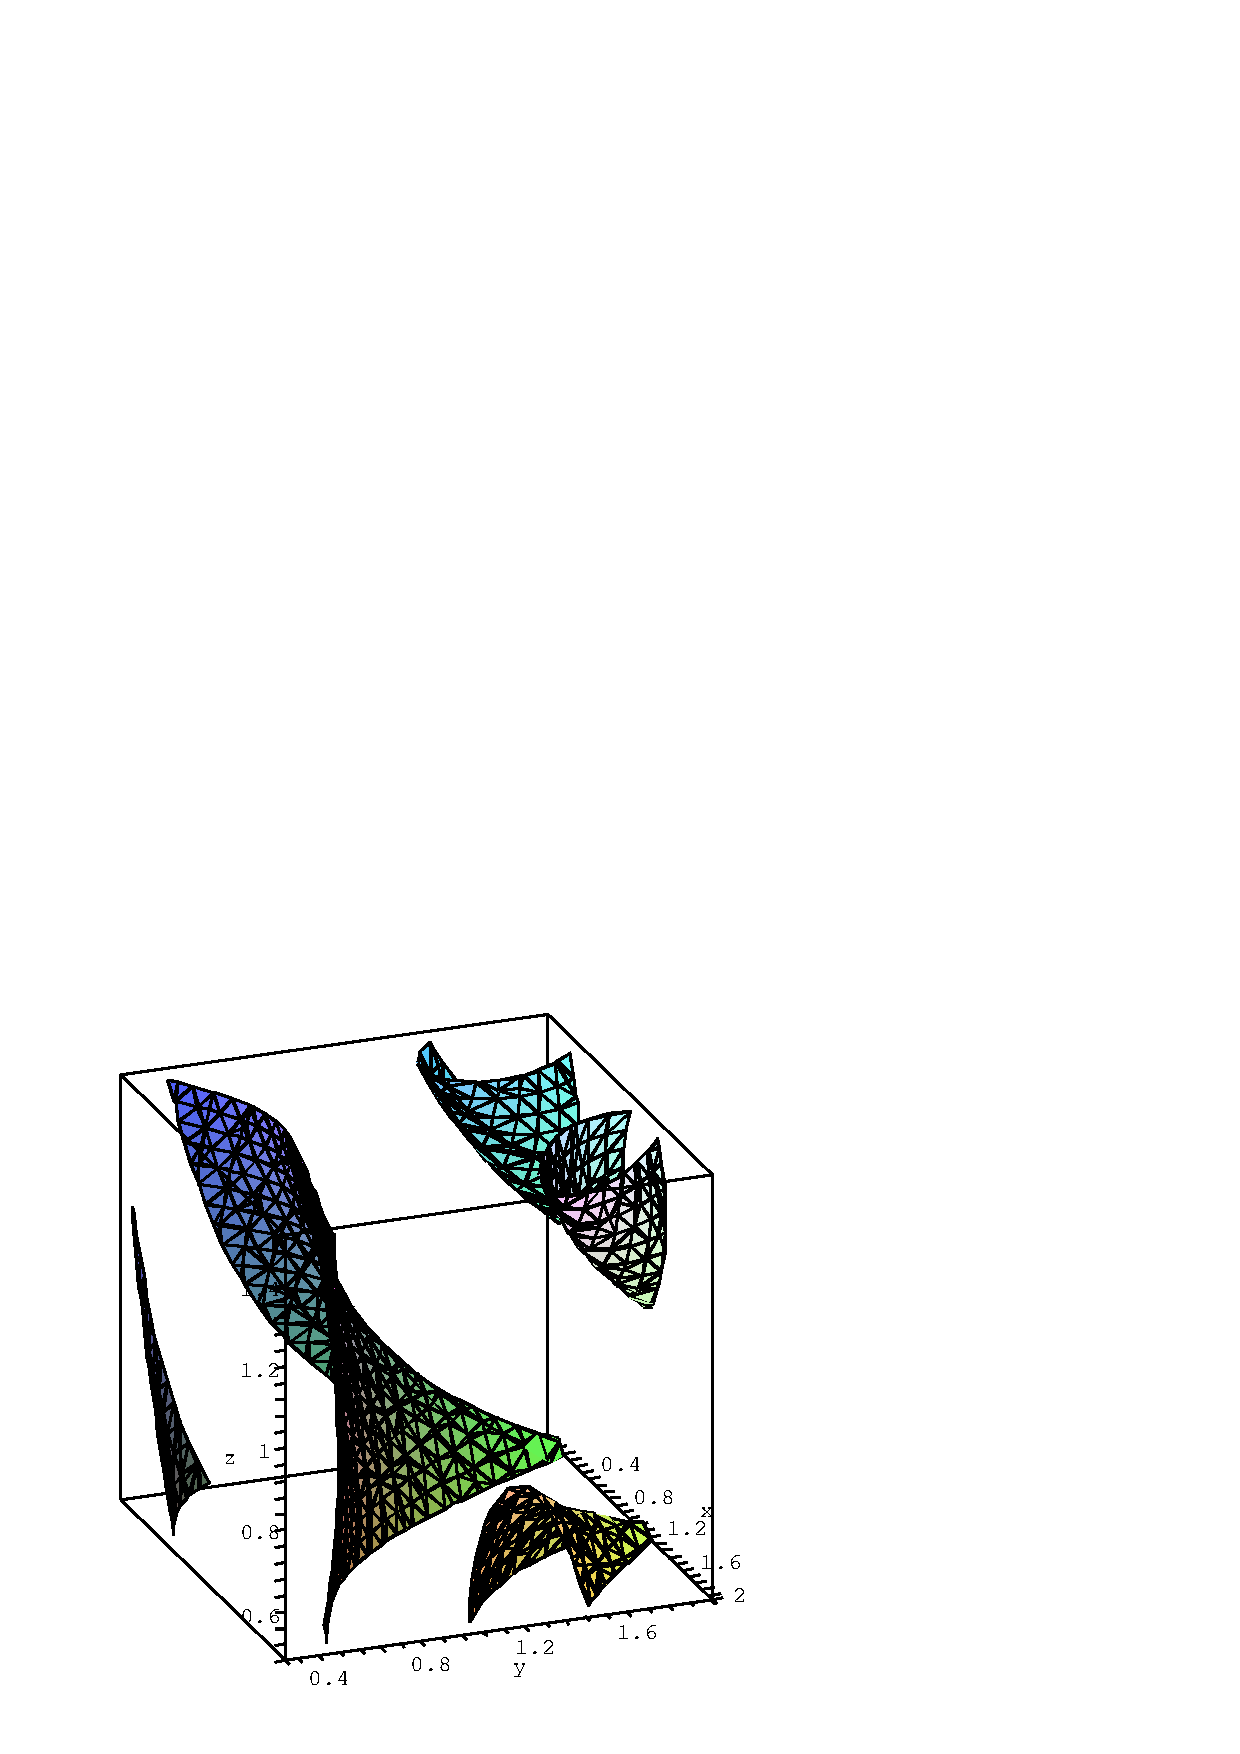
\includegraphics[height=8cm, keepaspectratio]{../images/pdf/jvNk-1.pdf}}
}
\indication{Le plan tangent \`a la surface d'\'equation $f(x,y,z)=0$ au point $(x_0,y_0,z_0)$ 
est donn\'e par l'\'equation
\begin{equation}
\frac{\partial f}{\partial x}(x_0,y_0,z_0) (x-x_0) +\frac{\partial f}{\partial y}(x_0,y_0,z_0)
(y-y_0)+\frac{\partial f}{\partial z}(x_0,y_0,z_0)(z-z_0) =0.
\label{tang4}
\end{equation}}
\reponse{
Soit $f\colon \R^3 \longrightarrow \R$ la fonction d\'efinie par
\[f(x,y,z)=\sin(\pi xy)+\sin(\pi yz) -1.\]
Ses d\'eriv\'ees partielles sont
\[\frac{\partial f}{\partial x} =\pi y \cos(\pi xy),\ 
\frac{\partial f}{\partial y} =\pi (x \cos(\pi xy) + z \cos(\pi yz)),
\ \frac{\partial f}{\partial y} =\pi y \cos(\pi yz)\]
et, apr\`es simplification, au point  $(1,\frac{1}{6}, 1)$, 
l'\'equation \eqref{tang4}  du plan tangent \`a la surface de niveau
en discussion devient
\[(x-1)+12(y-1/6)+(z-1)=0 .\]
Ainsi,  en ce point, le vecteur $(1,12,1)$ est perpendiculaire \`a la surface.
}
}
